\documentclass[12pt,english]{article}
\usepackage[english]{babel}
\usepackage{graphicx}
\usepackage{amsmath}
\usepackage{multirow}
\usepackage{pgfplots}
\usepackage{subcaption}
\usepackage{amssymb}
\usepackage[hidelinks]{hyperref}
\usepackage{caption}
\usepackage{amsthm}
\usepackage{multicol}
\pgfplotsset{compat=1.16}
\usepackage{minted}
\usepackage{float}
\usepackage{titling}
\usepackage{soul}
\usepackage{listings}
\newenvironment{statement}{\fontfamily{ptm}\selectfont}{\par}
\usepackage{array}
\graphicspath{ {../img/}}
\selectlanguage{english}
\usepackage[nottoc]{tocbibind}
\usepackage[utf8]{inputenc}
\usepackage{graphicx}
\usepackage[a4paper,left=2cm,right=2cm,top=2.5cm,bottom=2.5cm]{geometry}
\RecustomVerbatimEnvironment{Verbatim}{BVerbatim}{}


\title{Evolutionary Algorithms}
\setlength{\droptitle}{10em}
\author{Carlos Sánchez Páez}

\makeindex
\begin{document}


\begin{titlepage}

\newlength{\centeroffset}
\setlength{\centeroffset}{-0.5\oddsidemargin}
\addtolength{\centeroffset}{0.5\evensidemargin}
\thispagestyle{empty}

\noindent\hspace*{\centeroffset}
\begin{minipage}{\textwidth}

\centering

\includegraphics[width=0.75\textwidth]{bme_logo.jpg}\\[1.4cm]

\textsc{ \Large Evolutionary Algorithms\\[4cm]}

\textsc{\Huge Homework}\\[0.75cm]

{\Large\bfseries Fourth task\\}
\end{minipage}

\vspace{8cm}
\noindent\hspace*{\centeroffset}
\begin{minipage}{\textwidth}
\centering

\textbf{Author}\\ {Carlos Sánchez Páez}\\
\texttt{http://www.github.com/csp98}\\[0.5cm]
\textsc{Budapest University of Technology and Economics}\\
\vspace{1cm}
\textsc{Academic year 2018-2019}
\end{minipage}
\end{titlepage}
\thispagestyle{empty}

\newpage


\begin{enumerate}

	\item
		\begin{statement}
		Three individuals are coded $e_1 = 00010$, $e_2 = 01001$ and $e_3 = 11001$. How many schemes fits either $e_1$ or $e_2$? How many schemes fit all three?
		\end{statement}
		If we focus on $e_1$ and $e_2$, we can see that they differ only in positions 2,4 and 5. So the possible schemes are:
		\begin{itemize}
			\item 0\#0\#\#
			\item 0\#\#\#\#
			\item \#\#0\#\#
		\end{itemize}
		The schemes that fit all of them are:
		\begin{itemize}
			\item \#\#0\#\#
			\item \#\#\#\#\#
		\end{itemize}


	\item
		\begin{statement}
		Two individuals are coded $e_1 = 0101$ and $e_2 = 0100$. How many different offsprings can they have if we use one-point crossover? And if we use uniform crossover?
		\end{statement}
		As the individuals are equal in all their components (exept the last one), the possible offsprings will be two ($0101$ and $0100$) if we use one-point crossover.\\
		If we use uniform crossover, the result will be the same, as the first three components are always the same, no matter the parent we choose.


	\item
		\begin{statement}
		Find that largest codebook you can for the one error correcting codebook problem (using 8-long bit sequences as words).
		\end{statement}

		This problem can be easily solved by programming an script. It will
		calculate the possible binary combinations that can be made with $8$ bits. Then,
		it will add the items that have a hamming distance of at least $3$ to the codebook.
		Finally, we just have to calculate the lenght of the generated codebook.\\

		For $8$ bit words, the lenght of the codebook is $16$.

		\begin{figure}[H]
			\centering
			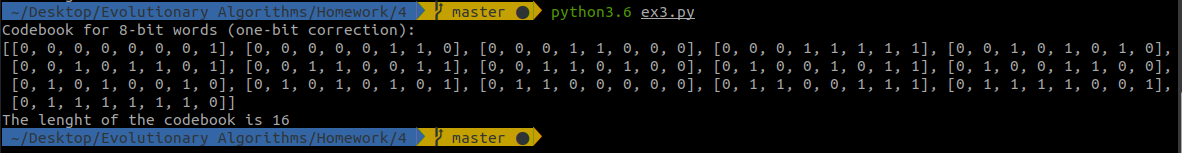
\includegraphics[scale=0.5]{ex3_output.png}
		\end{figure}


\end{enumerate}


\begin{thebibliography}{9}

\bibitem{Course Webpage}
Course Webpage
\\\texttt{http://math.bme.hu/~safaro/evolalgen.html}


\bibitem{Webpage4}
\texttt{https://tex.stackexchange.com/}


\end{thebibliography}


\end{document}
